%% Based on a TeXnicCenter-Template by Tino Weinkauf.
%%%%%%%%%%%%%%%%%%%%%%%%%%%%%%%%%%%%%%%%%%%%%%%%%%%%%%%%%%%%%

%%%%%%%%%%%%%%%%%%%%%%%%%%%%%%%%%%%%%%%%%%%%%%%%%%%%%%%%%%%%%
%% HEADER
%%%%%%%%%%%%%%%%%%%%%%%%%%%%%%%%%%%%%%%%%%%%%%%%%%%%%%%%%%%%%
\documentclass[a4paper,10pt]{report}
% Alternative Options:
%	Paper Size: a4paper / a5paper / b5paper / letterpaper / legalpaper / executivepaper
% Duplex: oneside / twoside
% Base Font Size: 10pt / 11pt / 12pt


%% Language %%%%%%%%%%%%%%%%%%%%%%%%%%%%%%%%%%%%%%%%%%%%%%%%%
\usepackage[USenglish]{babel} %francais, polish, spanish, ...
\usepackage[T1]{fontenc}
\usepackage[ansinew]{inputenc}

\usepackage{lmodern} %Type1-font for non-english texts and characters


%% Packages for Graphics & Figures %%%%%%%%%%%%%%%%%%%%%%%%%%
\usepackage{graphicx} %%For loading graphic files
%\usepackage{subfig} %%Subfigures inside a figure
%\usepackage{tikz} %%Generate vector graphics from within LaTeX

%% Please note:
%% Images can be included using \includegraphics{filename}
%% resp. using the dialog in the Insert menu.
%% 
%% The mode "LaTeX => PDF" allows the following formats:
%%   .jpg  .png  .pdf  .mps
%% 
%% The modes "LaTeX => DVI", "LaTeX => PS" und "LaTeX => PS => PDF"
%% allow the following formats:
%%   .eps  .ps  .bmp  .pict  .pntg


%% Math Packages %%%%%%%%%%%%%%%%%%%%%%%%%%%%%%%%%%%%%%%%%%%%
\usepackage{amsmath}
\usepackage{amsthm}
\usepackage{amsfonts}


%% Line Spacing %%%%%%%%%%%%%%%%%%%%%%%%%%%%%%%%%%%%%%%%%%%%%
%\usepackage{setspace}
%\singlespacing        %% 1-spacing (default)
%\onehalfspacing       %% 1,5-spacing
%\doublespacing        %% 2-spacing


%% Other Packages %%%%%%%%%%%%%%%%%%%%%%%%%%%%%%%%%%%%%%%%%%%
%\usepackage{a4wide} %%Smaller margins = more text per page.
%\usepackage{fancyhdr} %%Fancy headings
%\usepackage{longtable} %%For tables, that exceed one page


%%%%%%%%%%%%%%%%%%%%%%%%%%%%%%%%%%%%%%%%%%%%%%%%%%%%%%%%%%%%%
%% Remarks
%%%%%%%%%%%%%%%%%%%%%%%%%%%%%%%%%%%%%%%%%%%%%%%%%%%%%%%%%%%%%
%
% TODO:
% 1. Edit the used packages and their options (see above).
% 2. If you want, add a BibTeX-File to the project
%    (e.g., 'literature.bib').
% 3. Happy TeXing!
%
%%%%%%%%%%%%%%%%%%%%%%%%%%%%%%%%%%%%%%%%%%%%%%%%%%%%%%%%%%%%%

%%%%%%%%%%%%%%%%%%%%%%%%%%%%%%%%%%%%%%%%%%%%%%%%%%%%%%%%%%%%%
%% Options / Modifications
%%%%%%%%%%%%%%%%%%%%%%%%%%%%%%%%%%%%%%%%%%%%%%%%%%%%%%%%%%%%%

%\input{options} %You need a file 'options.tex' for this
%% ==> TeXnicCenter supplies some possible option files
%% ==> with its templates (File | New from Template...).
%---- Start Sourcecode formatting ----
\usepackage{listings}
\usepackage{courier}
\usepackage{caption}
\usepackage{color}
\usepackage{xcolor}

\lstloadlanguages{
  [Sharp]C,
  %Java
}

\lstset{
  basicstyle=\footnotesize\ttfamily, % Standardschrift
  %numbers=left,
  numberstyle=\tiny,
  %stepnumber=2,
  numbersep=5pt,
  tabsize=2,
  extendedchars=true,
  breaklines=true,
  frame=b,         
  keywordstyle=\color{blue}\bfseries,
  stringstyle=\color{red}\ttfamily,
  showspaces=false,
  showtabs=false,
  xleftmargin=17pt,
  framexleftmargin=17pt,
  framexrightmargin=5pt,
  framexbottommargin=4pt,
  %backgroundcolor=\color{lightgray},
  showstringspaces=false
 }

\DeclareCaptionFont{white}{\color{white}}
\DeclareCaptionFormat{listing}{\colorbox[cmyk]{0.43, 0.35, 0.35,0.01}{\parbox{\textwidth}{\hspace{15pt}#1#2#3}}}
\captionsetup[lstlisting]{format=listing,labelfont=white,textfont=white, singlelinecheck=false, margin=0pt, font={bf,footnotesize}}

%---- End Sourcecode formatting ----



%%%%%%%%%%%%%%%%%%%%%%%%%%%%%%%%%%%%%%%%%%%%%%%%%%%%%%%%%%%%%
%% DOCUMENT
%%%%%%%%%%%%%%%%%%%%%%%%%%%%%%%%%%%%%%%%%%%%%%%%%%%%%%%%%%%%%
\begin{document}

\pagestyle{empty} %No headings for the first pages.


%% Title Page %%%%%%%%%%%%%%%%%%%%%%%%%%%%%%%%%%%%%%%%%%%%%%%
%% ==> Write your text here or include other files.
%% Based on a TeXnicCenter-Template by Tino Weinkauf.
%%%%%%%%%%%%%%%%%%%%%%%%%%%%%%%%%%%%%%%%%%%%%%%%%%%%%%%%%%%%%

%%%%%%%%%%%%%%%%%%%%%%%%%%%%%%%%%%%%%%%%%%%%%%%%%%%%%%%%%%%%%
%% Deckblatt
%%%%%%%%%%%%%%%%%%%%%%%%%%%%%%%%%%%%%%%%%%%%%%%%%%%%%%%%%%%%%
%%
%% ATTENTION: You need a main file to use this one here.
%%            Use the command "\input{filename}" in your
%%            main file to include this file.
%%

\begin{titlepage}

\begin{center}

%\vspace*{1cm}
\Large
\textsc{Universiteit van Groningen}\\

\vspace{5cm}

%\LARGE
\textsc{Gevorderde Algoritmen en Datastructuren\\[0.5\baselineskip]
door\\[0.5\baselineskip]
Jos van der Til \& Rene Zuidhof}\\

\vspace{5cm}
\textsc{\today}\\ %%Date - better you write it yourself.

\vspace{1cm}
\end{center}

\end{titlepage}

%% Inhaltsverzeichnis %%%%%%%%%%%%%%%%%%%%%%%%%%%%%%%%%%%%%%%
\tableofcontents %Table of contents
\cleardoublepage %The first chapter should start on an odd page.

\pagestyle{plain} %Now display headings: headings / fancy / ...


%% Chapters %%%%%%%%%%%%%%%%%%%%%%%%%%%%%%%%%%%%%%%%%%%%%%%%%
%% ==> Write your text here or include other files.

%\input{intro} %You need a file 'intro.tex' for this.
% ********** Chapter 1 **********
\chapter{Introductie}
\label{sec:Hoofdstuk 1}

Een deel van de cursus Gevorderde Algoritmen en Datastructuren is een praticum, deze bestaat uit twee opdrachten. De eerste opdracht staat in dit document beschreven. Het doel van deze opdracht luidt: \textit{"ervaring opdoen met het analyseren en vergelijken van zoekalgoritmen. De opdracht sluit aan bij Chapter 3 van het leerboek Algorithm Design van Goodrich en Tamassia.
Het is de bedoeling om twee programma�s te ontwikkelen, waarmee je kunt bepalen welke
datastructuur beter is om een doorzoekbaar geordend lexicon (searchable ordered dictionary) te implementeren:
een conventionele binaire zoekboom, of een van de volgende alternatieve datastructuren:
AVL-boom, (2,4)-boom, splay tree, skip list. De programma�s dienen een tekstbestand woord voor
woord te lezen, waarbij elk nieuw woord wordt toegevoegd aan de datastructuur. Elk woord komt dus
slechts �e�enmaal voor in de datastructuur."}\\
\\
Een aantal van deze datastructuren staat beschreven in dit document, naast de beschrijving van de datastructuur is ook de uitkomst van de analyses die zijn uitgevoerd beschreven. In deze analyses is gekeken naar het aantal stringvergelijkingen, het aantal toekenningen in de code en de tijd die nodig is bij bepaalde handelingen.\\
\\
Als eerste zal in hoofdstuk 2 de conventionele binaire zoekboom behandeld worden. Hierna wordt gekeken naar gebalanceerde bomen, namelijk de AVL-boom (hoofdstuk 4) en de (2,4)-boom (hoofdstuk 5). Als laatste wordt in hoofdstuk 6 een alternatieve datastructuur behandeld, de skip list.\\
\\
In hoofdstuk 7 zal de analyse van al deze structuren behandeld worden.
\\
\section{Verwachting}

% ********** End of chapter **********

% ********** Chapter 2 **********
\chapter{Binaire zoekboom}
\label{sec:Hoofdstuk 2}

\begin{figure}[h]
	\centering
		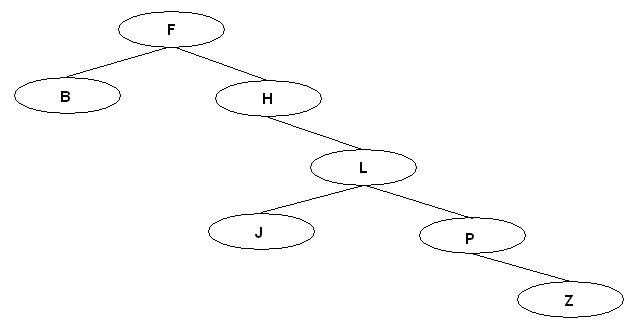
\includegraphics[width=\textwidth]{chap2/binarytree}
	\label{fig:binarytree}
\end{figure}

\section{Introductie}
Een van de simpelste zoekbomen is de binaire zoekboom. Elke interne knoop heeft twee kinderen waarvan de linkerkant lager is en de rechterkant hoger is dan de waarde in de interne knoop.\\
\\
\section{Zoeken}
Bij het zoeken naar een waarde $k$ in een binaire boom wordt begonnen in de root knoop. Als $k$ kleiner is dan de waarde in de knoop $p$ wordt verder gezocht in het linkerkind van $p$. Wanneer $k$ groter is dan de waarde in $p$ wordt verder gezocht in het rechterkind van $p$. Dit wordt gedaan tot een externe knoop is bereikt of wanneer $k$ gevonden is.\\
\\
\section{Toevoegen}
Met behulp van bovenstaande zoek methode wordt gezocht naar de toe te voegen waarde $k$. Wanneer de gevonden waarde $p$ een interne knoop is wordt er direct gestopt met toevoegen, $k$ zit namelijk al in de boom. Wanneer $p$ een externe knoop is wordt deze vervangen door $k$ en worden twee externe kinderen toegevoegd aan $k$.\\
\\
\section{Analyse}

% ********** End of chapter **********
% ********** Chapter 3 **********
\chapter{AVL-boom}
\label{sec:Hoofdstuk 3}

% ********** End of chapter **********
% ********** Chapter 4 **********
\chapter{AVL-boom}
\label{sec:Hoofdstuk 4}

% ********** End of chapter **********
% ********** Chapter 5 **********
\chapter{(2,4)-boom}
\label{sec:Hoofdstuk 5}

Intro
De tweede gebalanceerde boom die behanded wordt is de (2,4)-boom. Alle interne knopen van deze boom hebben ��n tot drie keys, het aantal kinderen van een knoop is het aantal keys + 1. Dit betekent dus dat elke knoop 2, 3 of 4 kinderen heeft, vandaar de naam (2,4)-boom (soms ook (2,3,4)-boom genoemd). Een andere eigenschap van deze boom is dat de diepte van alle externe knopen gelijk is. Deze eigenschappen zorgen ervoor dat de hoogte van een (2,4)-boom met $n$ items $\Theta(log n)$ is. Deze eigenschappen worden bewaard door na elke toevoeging of verwijdering te kijken of de boom gebalanceerd moet worden. De boom moet gebalanceerd worden wanneer een knoop in de boom geen keys (woorden) meer bevat of wanneer een knoop meer dan drie keys bevat.

Balanceren
Omdat bij deze analyse alleen gekeken wordt naar het toevoegen van keys zal de boom alleen gebalanceerd worden wanneer een knoop meer dan drie keys bevat. Wanneer een knoop meer dan drie keys bevat (overflow), zal de boom gebalanceerd moeten worden.
Dit wordt gedaan door de derde waarde van de knoop met meer dan drie keys toe te voegen aan zijn parent. De eerste twee keys worden dan het kind aan de linkerkant van toegevoegde key in de parent en de vierde waarde het kind aan de rechterkant.

Zoeken
Bij het searchen van een key zal begonnen worden bij de root knoop. Als de knoop niet de gezochte key bevat zal gekeken worden in het kind voor de key die lager is dan de invoer. Dit wordt gedaan tot een externe knoop is bereikt of tot een knoop is bereikt die de invoer bevat.

Toevoegen
Bij het toevoegen zal eerst gezocht worden op de bovenstaande manier. Wanneer een knoop wordt gevonden die de key al bevat zal gestopt worden met toevoegen. Als dit niet het geval is, we hebben dan dus een externe knoop, zal de waarde toegevoegd worden aan de parent. Hierna zal de balance methode aangeroepen worden om te kijken of de boom ongebalanceerd is en balanceren wanneer dit het geval is.

Analyse


% ********** End of chapter **********
% ********** Chapter 6 **********
\chapter{Skip List}
\label{sec:Hoofdstuk 6}

\begin{figure}[h]
	\centering
		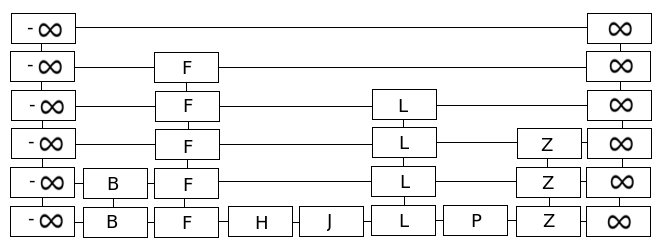
\includegraphics[width=\textwidth]{chap6/skiplist}
	\label{fig:skiplist}
\end{figure}

\section{Introductie}
Naast bomen zijn er ook andere manieren om zoekalgoritmen te implementeren. In dit hoofdsuk zal een van deze structuren behandeld worden, namelijk de skip list. Een skip list bestaat uit een aantal lijsten waarvan elke lijst een subset van de lijst onder hem bevat. De onderste lijst bevat alles waardes van de boom. Elke lijst bevat in ieder geval de waardes -\infty en \infty. Hierdoor zullen alle waardes in de lijst tussen deze twee waardes in zitten.\\
\\
\section{Zoeken}
Bij het zoeken naar een waarde $k$ in een skiplist wordt begonnen in de meest linkse waarde in de bovenste lijst, deze waarde noemen we $p$. Hierna zal gekeken worden in de waarde onder $p$, als deze niet leeg is wordt dit de nieuwe waarde van $p$. Vervolgens wordt gekeken naar de waardes aan de rechterkant van $p$. Er wordt naar rechts gezocht tot er een waarde gevonden wordt hoger dan $k$, $p$ wordt nu de waarde voor de laatst gevonde waarde. Dit wordt gedaan tot de gezochte waarde wordt gevonden. Wanneer $k$ niet in de skip list zit wordt de hoogst mogelijke waarde voor $k$ gereturned.\\
\\
\section{Toevoegen}
Bij het toevoegen van waarde $k$ wordt eerst gezocht naar $k$ op de manier zoals hierboven beschreven is. Als de gevonden waarde $p$ gelijk is aan $k$ zal direct gestopt worden, de waarde zit namelijk al in de skip list. Wanneer deze niet gelijk is zal de waarde toegevoegd worden na $p$. Hierna zal $k$ toegevoegd worden zolang een random getal tussen de 0 en 1 lager is dan 0.5.\\
\\
\section{Verwijderen}
Bij het verwijderen van een waarde $k$ zal eerst gezocht worden op deze waarde. Als de gevonden waarde $p$ niet gelijk is aan $k$ zal direct gestopt worden, $k$ zit niet in de skip list. Wanneer $k$ en $p$ wel gelijk zijn zal $p$ verwijderd worden samen met alle waardes boven $p$.\\
\\
\section{Analyse}

% ********** End of chapter **********
% ********** Chapter 7 **********
\chapter{Conclusie}
\label{sec:Hoofdstuk 7}



% ********** End of chapter **********
% ********** Chapter 8 **********
\chapter{Conclusie}
\label{sec:Hoofdstuk 8}



% ********** End of chapter **********
%%%%%%%%%%%%%%%%%%%%%%%%%%%%%%%%%%%%%%%%%%%%%%%%%%%%%%%%%%%%%
%% BIBLIOGRAPHY AND OTHER LISTS
%%%%%%%%%%%%%%%%%%%%%%%%%%%%%%%%%%%%%%%%%%%%%%%%%%%%%%%%%%%%%
%% A small distance to the other stuff in the table of contents (toc)
\addtocontents{toc}{\protect\vspace*{\baselineskip}}

%% The Bibliography
%% ==> You need a file 'literature.bib' for this.
%% ==> You need to run BibTeX for this (Project | Properties... | Uses BibTeX)
%\addcontentsline{toc}{chapter}{Bibliography} %'Bibliography' into toc
%\nocite{*} %Even non-cited BibTeX-Entries will be shown.
%\bibliographystyle{alpha} %Style of Bibliography: plain / apalike / amsalpha / ...
%\bibliography{literature} %You need a file 'literature.bib' for this.

%% The List of Figures
\clearpage
\addcontentsline{toc}{chapter}{List of Figures}
\listoffigures

%% The List of Tables
%\clearpage
%\addcontentsline{toc}{chapter}{List of Tables}
%\listoftables


%%%%%%%%%%%%%%%%%%%%%%%%%%%%%%%%%%%%%%%%%%%%%%%%%%%%%%%%%%%%%
%% APPENDICES
%%%%%%%%%%%%%%%%%%%%%%%%%%%%%%%%%%%%%%%%%%%%%%%%%%%%%%%%%%%%%
\appendix
%% ==> Write your text here or include other files.

%\input{FileName} %You need a file 'FileName.tex' for this.
\chapter{Main classes}
\lstset{language=Java}
\begin{lstlisting}[caption=Main classes Source code - Main]
public class Main {

	/**
	 * @param args
	 */
	public static void main(String[] args) {
		String[] textFiles = new String[] { "text1", "text2", "text3", "text4",
				"text5" };
		TextSource tx = new TextSource();

		tx.preloadAll();
		try {
			PrintStream output = new PrintStream(new FileOutputStream(
					"bench_results.txt"));
			System.setOut(output);
		} catch (IOException ioe) {
			ioe.printStackTrace();
			System.exit(-1);
		}

		for (int i = 0; i < 10; i++) {
			System.out.printf("Start of run %d....\n", i);
			Profiler p = new Profiler();

			ITree tree;

			System.out.println("\nBinaryTree");
			for (String s : textFiles) {
				tree = new TreeImpl(p);
				test(tree, p, tx, s);
				p.reset(true);
			}

			System.out.println("AVLTree");
			for (String s : textFiles) {
				tree = new AVLTree(p);
				test(tree, p, tx, s);
				p.reset(true);
			}

			System.out.println("\nSkipList");
			for (String s : textFiles) {
				tree = new SkipList(p);
				test(tree, p, tx, s);
				p.reset(true);
			}

			System.out.println("\n2-4 Tree");
			for (String s : textFiles) {
				tree = new TwoFourTree(p);
				test(tree, p, tx, s);
				p.reset(true);
			}

			System.out.println("End of run");
		}
		
		System.out.flush();
		System.out.close();
	}

	private static void test(ITree tree, Profiler p, TextSource tx,
			String textFile) {
		StopWatch st = new StopWatch();
		String insertionTimerName = String.format("Insertion %s", textFile);

		st.start(insertionTimerName);
		for (String s : tx.getTextFile(textFile)) {
			tree.insert(s);
		}
		st.stop(insertionTimerName);

		System.out.println("Insertion");
		p.printInfo();

		p.reset(true);

		String searchTimerName = String.format("Search %s", textFile);

		st.start(searchTimerName);
		for (String s : tx.getTextFile(textFile)) {
			tree.getNode(s);
		}
		st.stop(searchTimerName);

		System.out.println("Search");
		p.printInfo();

		st.printTimers();
	}
}

\end{lstlisting}

\begin{lstlisting}[caption=Main classes Source code -ITree]
/*
 * Interface for all structures used in this project
 */
public interface ITree {
	
	/*
	 * Searches the structure for parameter key
	 * Returns the node containing the key or returns the node closest to key
	 */
	ITreeNode getNode(String key);
	
	/*
	 * Insert string into structure
	 * Returns the node containing key after insertion
	 */
	ITreeNode insert(String key);
}

\end{lstlisting}

\begin{lstlisting}[caption=Main classes Source code - ITreeNode]
public interface ITreeNode {

	/*
	 * Returns the value of this node
	 */
	public String getKey();
}
\end{lstlisting}
\chapter{Util classes}
\lstset{language=Java}
\begin{lstlisting}[caption=Util classes Source code - Profiler]
public class Profiler {

	public static final Profiler NULL = new NullProfiler();
	
	private static final class NullProfiler extends Profiler {
		public Profiler incAssignments() { return this;}
		public Profiler addAssignments(long assignments) { return this;}
		public Profiler incComparisons() {return this; }
		public Profiler addComparisons(long comparisons) {return this; }
	}
	
	private long comparisons;
	private long assignments;
	
	public Profiler incAssignments() {
		++assignments;
		
		return this;
	}
	
	public Profiler addAssignments(long assignments) {
		this.assignments += assignments;
		
		return this;
	}
	
	public Profiler incComparisons() {
		++comparisons;
		
		return this;
	}
	
	public Profiler addComparisons(long comparisons) {
		this.comparisons += comparisons;
		
		return this;
	}
	
	public void reset(boolean reset) {
		if(reset) {
			comparisons = 0;
			assignments = 0;
		}
	}

	public void printInfo() {
		System.out.printf("Comparisons: %d\nAssignments: %d\n", comparisons, assignments);
	}
}
\end{lstlisting}

\begin{lstlisting}[caption=Util classes Source code - StopWatch]
public class StopWatch {

	private Map<String, StopWatchInfo> stopWatchMap;
	
	public StopWatch() {
		stopWatchMap = new HashMap<String, StopWatchInfo>();
	}
	
	public void start(String name) {
		StopWatchInfo info = new StopWatchInfo();
		
		stopWatchMap.put(name, info);
		
		info.startTime = System.currentTimeMillis();
	}
	
	public void stop(String name) {
		long stop = System.currentTimeMillis();
		
		StopWatchInfo info = stopWatchMap.get(name);
		
		info.stopTime = stop;
	}
	
	public void printTimers() {
		for(Entry<String, StopWatchInfo> entry : stopWatchMap.entrySet()) {
			System.out.printf("------%s------\n", entry.getKey());
			System.out.printf("-- Run time: %d ms.\n", getTimeMillis(entry.getKey()));
		}
			
	}
	
	public long getTimeMillis(String name) {
		StopWatchInfo info = stopWatchMap.get(name);
		
		if(info.stopTime == 0)
			return System.currentTimeMillis() - info.startTime;
		
		return info.stopTime - info.startTime;
	}
	
	private class StopWatchInfo {
		public long startTime;
		public long stopTime;
	}
}
\end{lstlisting}

\begin{lstlisting}[caption=Util classes Source code - TextSource]
public class TextSource {

	private Map<String, List<String>> textFiles;
	
	public TextSource() {
		textFiles = new HashMap<String, List<String>>();
	}
	
	public List<String> getTextFile(String name) {
		if(!textFiles.containsKey(name)) {
			BufferedReader reader = null;
			
			try {
				reader = new BufferedReader(new FileReader(name));
				List<String> list = new LinkedList<String>();
				
				
				String line;
				while((line = reader.readLine()) != null) {
					String[] split = line.split(" ");
					
					Collections.addAll(list, split);
				}
				
				textFiles.put(name, list);
			} catch(IOException ioe) {
				ioe.printStackTrace();
				System.exit(-1);
			} finally {
				try {
					reader.close();
				} catch(Exception e) {/* Ignored, we are destroying anyway */}
			}
		}
		
		return textFiles.get(name);
	}

	public void preloadAll() {
		getTextFile("text1");
		getTextFile("text2");
		getTextFile("text3");
		getTextFile("text4");
		getTextFile("text5");
	}
}
\end{lstlisting}
\chapter{BinaryTree classes}
\lstset{language=Java}
\begin{lstlisting}[caption=BinaryTree classes Source code - TreeImpl]
public class TreeImpl implements ITree {
	private TreeNode root;
	
	private Profiler profiler;
	
	public TreeImpl() {
		this(Profiler.NULL);
	}
	
	public TreeImpl(Profiler p) {
		this.profiler = p;
	}

	@Override
	public TreeNode getNode(String key) {
		TreeNode next = root;
		profiler.incAssignments();
		
		int comp;

		while (next != null) {
			comp = key.compareTo(next.key);
			
			profiler.incComparisons()
					.incAssignments();
			
			if (comp == 0)
				return next;
			else if (comp < 0) {
				next = next.left;
				profiler.incAssignments();
			}
			else {
				next = next.right;
				profiler.incAssignments();
			}
		}

		return null;
	}

	@Override
	public TreeNode insert(String key) {
		TreeNode node = getNode(key);
		
		profiler.incAssignments();
		
		if (node != null)
			return node;

		if (root == null) {
			root = new TreeNode(key);
			profiler.incAssignments();
		} else {
			boolean inserted = false;
			TreeNode current = root;
			
			profiler.addAssignments(2);
			
			int compRes;

			while (!inserted) {
				compRes = key.compareTo(current.key);
				profiler.incComparisons().incAssignments();
				
				if (compRes < 0 && current.left == null) {
					// Smaller, and left child is free. Insert
					current.left = new TreeNode(key);
					current.left.parent = current;
					inserted = true;
					
					profiler.addAssignments(3);
				} else if (compRes < 0 && current.left != null) {
					// Smaller, but left child is not free. Continue.
					current = current.left;
					profiler.incAssignments();
				} else if (compRes > 0 && current.right == null) {
					// Bigger, and right child is free. Insert
					current.right = new TreeNode(key);
					current.right.parent = current;
					inserted = true;
					
					profiler.addAssignments(3);
				} else {
					// Bigger, and right child is not free. Continue
					current = current.right;
					
					profiler.incAssignments();
				}
			}
		}
		
		return null;
	}
}
\end{lstlisting}

\begin{lstlisting}[caption=BinaryTree classes Source code - TreeNode]
public class TreeNode implements Comparable<TreeNode>, ITreeNode {

	public String key;
	public TreeNode parent;
	public TreeNode left;
	public TreeNode right;
	
	public TreeNode(String key) {
		this.key = key;
	}

	@Override
	public int compareTo(TreeNode t) {
		return this.key.compareTo(t.key);
	}
	
	public boolean isLeaf() {
		return childCount() == 0;
	}
	
	public int childCount() {
		int count = 0;
		
		if(left != null)
			count++;
		
		if(right != null)
			count++;
		
		return count;
	}

	@Override
	public String getKey() {
		return key;
	}
}
\end{lstlisting}
\chapter{AVL-Tree classes}
\lstset{language=Java}
\begin{lstlisting}[caption=AVL-Tree classes Source code - AVLTree]
public class AVLTree implements ITree {

	private AVLNode root;
	private AVLNode first; /* Left most node */
	private AVLNode last; /* Right most node */
	private int height;
	
	private Profiler profiler;
	
	public AVLTree() {
		this(Profiler.NULL);
	}
	
	public AVLTree(Profiler p) {
		profiler = p;
	}
	
	@Override
	public AVLNode getNode(String key) {
		return findInsertionPoint(key).node;
	}
	
	private class InsertionInfo {
		public AVLNode node;
		public AVLNode parent;
		public AVLNode unbalanced;
		public boolean isLeft;
	}
	
	private InsertionInfo findInsertionPoint(String key) {
		AVLNode node = root;
		int cmpRes = 0;
		
		profiler.addAssignments(2);
		
		InsertionInfo result = new InsertionInfo();
		
		result.node = null;
		result.unbalanced = node;
		result.isLeft = false;
		result.parent = null;
		
		profiler.addAssignments(4);
		
		while(node != null) {
			if(node.getBalance() != 0)
				result.unbalanced = node;
			
			cmpRes = node.getKey().compareTo(key);
			profiler.incComparisons();
			profiler.incAssignments();
			
			if(cmpRes == 0) { /* Node key is equal to key */
				result.node = node;
				profiler.incAssignments();
				return result;
			}
			
			profiler.incAssignments();
			result.parent = node; /* 
								   * Assignment done here. This is because if the key is found at the first iteration, the key is in the root node. 
								   * Root nodes don't have parents. Saves an assignment.
								   */
			
			if((result.isLeft = cmpRes > 0)) { /* Node is smaller then key, go left. Save this */
				node = node.getLeft();
			} else {
				node = node.getRight();
			}
			
			profiler.incAssignments();
		}
		
		return result;
	}
	
	/* Balancing functions */
	private void rotateLeft(AVLNode node) {
		/*
		 * Let Q be P's right child.
		 * Set Q to be the new root.
		 * Set P's right child to be Q's left child.
		 * Set Q's left child to be P.
		 */
		AVLNode p = node; /* Pivot node */
		AVLNode q = node.getRight();
		AVLNode parent = node.getParent();
		
		profiler.addAssignments(3);
		
		if(!p.isRoot()) {
			if(parent.getLeft() == p)
				parent.setLeft(q);
			else
				parent.setRight(q);
		} else {
			root = q;
		}
		
		profiler.incAssignments();
		
		q.setParent(parent);
		p.setParent(q);
		p.setRight(q.getLeft());
		
		profiler.addAssignments(3);
		
		if(p.hasRight()) {
			p.getRight().setParent(p);
			profiler.incAssignments();
		}
		
		q.setLeft(p);
		
		profiler.incAssignments();
	}
	
	private void rotateRight(AVLNode node) {
		/* 
		 * Let P be Q's left child.
		 * Set P to be the new root.
		 * Set Q's left child to be P's right child.
		 * Set P's right child to be Q.
		 */
		AVLNode q = node; /* Pivot node */
		AVLNode p = node.getLeft();
		AVLNode parent = q.getParent();
		
		profiler.addAssignments(3);
		
		if(!q.isRoot()) {
			if(parent.getLeft() == q)
				parent.setLeft(p);
			else
				parent.setRight(p);
		} else {
			root = p;
		}
		
		profiler.incAssignments();
		
		p.setParent(parent);
		q.setParent(p);
		q.setLeft(p.getRight());
		
		profiler.addAssignments(3);
		
		if(q.hasLeft()) {
			q.getLeft().setParent(q);
			
			profiler.incAssignments();
		}
		
		p.setRight(q);
		
		profiler.incAssignments();
	}

	@Override
	public AVLNode insert(String key) {
		InsertionInfo info = findInsertionPoint(key);
		
		profiler.incAssignments();
		
		if(info.node != null) /* Key already in tree. Return node. */
			return info.node;
		
		AVLNode node = new AVLNode(key);
		
		profiler.incAssignments();
		
		if(info.parent == null) { /* No root */
			root = node;
			first = last = node;
			height++;
			
			profiler.addAssignments(4);
			return null;
		}
		
		AVLNode parent = info.parent;
		
		profiler.incAssignments();
		
		if(info.isLeft) {
			if(parent == first) {
				first = node;
				profiler.incAssignments();
			}
		} else {
			if(parent == last) {
				last = node;
				profiler.incAssignments();
			}
		}
		
		node.setParent(parent);
		
		if(info.isLeft) {
			parent.setLeft(node);
		} else {
			parent.setRight(node);
		}
		
		AVLNode unbalanced = info.unbalanced;
		
		profiler.addAssignments(3);
		
		for(;;) { /* Update balance values. */
			if(parent.getLeft() == node)
				parent.decBalance();
			else
				parent.incBalance();
			
			profiler.incAssignments();
			
			if(parent == unbalanced)
				break;
			
			node = parent;
			parent = parent.getParent();
			
			profiler.addAssignments(2);
		}
		
		switch(unbalanced.getBalance()) {
		case 1:
			/* fall through */
		case -1:
			height++; /* Update tree height */
			profiler.incAssignments();
			/* fall through */
		case 0:
			break;
			
		case 2: /* Tree unbalanced to the right. */
			AVLNode right = unbalanced.getRight();
			
			profiler.incAssignments();
			
			if(right.getBalance() == 1) {
				unbalanced.setBalance(0);
				right.setBalance(0);
				
				profiler.addAssignments(2);
			} else {
				switch(right.getLeft().getBalance()) {
				case 1:
					unbalanced.setBalance(-1);
					right.setBalance(0);
					profiler.addAssignments(2);
					break;
				case 0:
					unbalanced.setBalance(0);
					right.setBalance(0);
					profiler.addAssignments(2);
					break;
				case -1:
					unbalanced.setBalance(0);
					right.setBalance(1);
					profiler.addAssignments(2);
					break;
				}
				
				right.getLeft().setBalance(0);
				
				profiler.incAssignments();
				
				rotateRight(right);
			}
			rotateLeft(unbalanced);
			break;
			
		case -2: /* Tree unbalanced to the left. */
			AVLNode left = unbalanced.getLeft();
			
			profiler.incAssignments();
			
			if(left.getBalance() == -1) {
				unbalanced.setBalance(0);
				left.setBalance(0);
				
				profiler.addAssignments(2);
			} else {
				switch(left.getRight().getBalance()) {
				case 1:
					unbalanced.setBalance(0);
					left.setBalance(-1);
					profiler.addAssignments(2);
					break;
				case 0:
					unbalanced.setBalance(0);
					left.setBalance(0);
					profiler.addAssignments(2);
					break;
				case -1:
					unbalanced.setBalance(1);
					left.setBalance(0);
					profiler.addAssignments(2);
					break;
				}
				left.getRight().setBalance(0);
				
				profiler.incAssignments();
				
				rotateLeft(left);
			}
			rotateRight(unbalanced);
			break;
		}
		
		return null;
	}
}
\end{lstlisting}

\begin{lstlisting}[caption=AVLTree classes Source code - AVLNode]
public class AVLNode implements ITreeNode {

	private AVLNode parent;
	private AVLNode left;
	private AVLNode right;

	private String key;

	private int balance; /* Range: -2 -> +2 */

	public AVLNode(String key) {
		this.key = key;
		parent = null;
		left = null;
		right = null;
	}

	/* Start balance methods */
	
	public int getBalance() {
		return balance;
	}

	public void setBalance(int balance) {
		this.balance = balance;
	}

	public void incBalance() {
		++this.balance;
	}

	public void decBalance() {
		--this.balance;
	}

	/* End balance methods */

	/* Node methods */
	public AVLNode getParent() {
		return parent;
	}

	public void setParent(AVLNode parent) {
		this.parent = parent;
	}
	
	public boolean isRoot() {
		return parent == null;
	}
	
	public AVLNode getLeft() {
		return left;
	}

	public void setLeft(AVLNode left) {
		this.left = left;
	}

	public AVLNode getRight() {
		return right;
	}

	public void setRight(AVLNode right) {
		this.right = right;
	}

	public boolean hasLeft() {
		return left != null;
	}

	public boolean hasRight() {
		return right != null;
	}

	/* Key methods */

	public String getKey() {
		return key;
	}

	public void setKey(String key) {
		this.key = key;
	}
}
\end{lstlisting}
\chapter{(2,4)-Tree classes}
\lstset{language=Java}
\begin{lstlisting}[caption=TwoFourTree classes Source code - TwoFourTree]
public class TwoFourTree implements ITree {

	private TwoFourNode root;
	private Profiler profiler;
	
	public TwoFourTree(Profiler p){
		root = new TwoFourNode(p);
		TwoFourNode external = new TwoFourNode(p);
		external.setExternal(true);
		external.setParent(root);
		root.addChild(external, 0, false);
		
		profiler = p;
	}
	
	public TwoFourTree() {
		this(Profiler.NULL);
	}
	
	public TwoFourNode insert(String text){
		TwoFourNode node = getNode(text);
		
		profiler.incAssignments();
		
		if(node.contains(text)){
			return node;
		}
		
		
		if(node.isExternal()){
			node = node.getParent();
			int index = node.addValue(text);
			TwoFourNode external = new TwoFourNode(profiler);
			
			external.setExternal(true);
			external.setParent(node);
			
			profiler.addAssignments(3);
			
			node.addChild(external, index + 1, false);
			rebalance(node);
		}
		
		return null;
	}
	
	private void rebalance(TwoFourNode node){
		if(node.getValueCount() > 3){
			TwoFourNode u;
			
			if(node.equals(root)){
				root = new TwoFourNode(profiler);
				u = root;
				
				profiler.addAssignments(2);
			} else {
				u = node.getParent();
				
				profiler.incAssignments();
			}
			
			TwoFourNode node1 = new TwoFourNode(profiler);
			profiler.incAssignments();
			
			node1.addValue(node.getValues().get(0));
			node1.addValue(node.getValues().get(1));
			
			if(node.getChildrenCount() == 0){
				TwoFourNode external1 = new TwoFourNode(profiler);
				profiler.incAssignments();
				
				external1.setExternal(true);
				external1.setParent(node1);
				node1.addChild(external1, 0, false);
				node1.addChild(external1, 1, false);
				node1.addChild(external1, 2, false);
			} else {
				node1.addChild(node.getChild(0), 0, false);
				node1.addChild(node.getChild(1), 1, false);
				node1.addChild(node.getChild(2), 2, false);
				node.getChild(0).setParent(node1);
				node.getChild(1).setParent(node1);
				node.getChild(2).setParent(node1);
			}
			
			TwoFourNode node2 = new TwoFourNode(profiler);
			profiler.incAssignments();
			
			node2.addValue(node.getValues().get(3));
			if(node.getChildrenCount() == 0){
				TwoFourNode external2 = new TwoFourNode(profiler);
				external2.setExternal(true);
				external2.setParent(node2);
				node2.addChild(external2, 0, false);
				node2.addChild(external2, 1, false);
			} else {
				node2.addChild(node.getChild(3), 0, false);
				node2.addChild(node.getChild(4), 1, false);
				node.getChild(3).setParent(node2);
				node.getChild(4).setParent(node2);
			}

			int index = u.addValue(node.getValues().get(2));
			profiler.incAssignments();
			
			u.addChild(node1, index, true);
			node1.setParent(u);
			u.addChild(node2, index + 1, false);
			node2.setParent(u);
			rebalance(u);			
		}
	}
	
	public TwoFourNode getNode(String text){
		TwoFourNode node = root;
		profiler.incAssignments();
		
		while(!node.contains(text) && !node.isExternal()){
			int i = 0;
			profiler.incAssignments();
			
			for(String s : node.getValues()){
				if(s != null){
					if(s.compareTo(text) < 0){
						i++;
						profiler.incAssignments();
					}
					profiler.incComparisons();
				}
			}
			
			node = node.getChild(i);
			profiler.incAssignments();
		}
		
		return node;
	}
}
\end{lstlisting}

\begin{lstlisting}[caption=TwoFourTree classes Source code - TwoFourNode]
public class TwoFourNode implements ITreeNode {

	private LinkedList<String> valuesList = new LinkedList<String>();
	private LinkedList<TwoFourNode> childrenList = new LinkedList<TwoFourNode>();
	private TwoFourNode parent = null;
	
	private Profiler profiler;
	
	private boolean external = false;
	
	public TwoFourNode(Profiler p) {
		profiler = p;
	}
	
	public String getKey() {
		throw new IllegalAccessError("Use cast & getValues, damn 2-4 trees...");
	}
	
	public int addValue(String text){
		int index = 0;
		profiler.incAssignments();
		
		for(String s : valuesList){
			if(s != null){
				profiler.incComparisons();
				if(s.compareTo(text) <= 0) {
					index++;
					profiler.incAssignments();
				}
			}
		}
		
		valuesList.add(index, text); 		//Counted as 1 assignment.
		profiler.incAssignments();
		
		return index;
	}
	
	public List<String> getValues() {
		return valuesList;
	}
	
	public int getValueCount(){
		int count = 0;
		for(String s : valuesList){
			if(s != null){
				profiler.incAssignments();
				count++;
			}
		}
		return count;
	}
	
	public void removeValue(String text){
		valuesList.remove(text); //Counted as 1 assignment.
		
		profiler.incAssignments();
	}
	
	public int getChildrenCount(){
		return childrenList.size();
	}
	
	public boolean contains(String text){
		for(String s : valuesList) {
			profiler.incComparisons();
			
			if(s.equals(text))
				return true;
		}
		
		return false;
	}
	
	/*
	 * if replace is true the child will will be replaced by the new child
	 * else the other childs will shift one to the right
	 */
	public void addChild(TwoFourNode child, int number, boolean replace){		
		if(replace && childrenList.size() > 0){
			childrenList.remove(number); //Counted as 1 assignment.
			profiler.incAssignments();
		}
		
		childrenList.add(number, child); //Counted as 1 assignment.
		profiler.incAssignments();
	}
	
	public TwoFourNode getChild(int number){
		return childrenList.get(number);
	}
	
	public List<TwoFourNode> getChildren(){
		return childrenList;
	}

	public void setParent(TwoFourNode parent) {
		this.parent = parent;
		profiler.incAssignments();
	}

	public TwoFourNode getParent() {
		return parent;
	}

	public void setExternal(boolean external) {
		this.external = external;
		profiler.incAssignments();
	}

	public boolean isExternal() {
		return external;
	}
}
\end{lstlisting}
\chapter{Skip List classes}
\lstset{language=Java}
\begin{lstlisting}[caption=Skip List classes Source code - SkipList]
public class SkipList implements ITree {

	private SkipNode first = new SkipNode("");
	private SkipNode last = new SkipNode("");

	private Profiler profiler;

	public SkipList(Profiler p) {
		first.setIsFirst();
		last.setIsLast();
		first.setAfter(last);
		last.setBefore(last);

		profiler = p;
	}

	public SkipList() {
		this(Profiler.NULL);
	}

	public ITreeNode insert(String text) {
		SkipNode p = getNode(text);
		
		profiler.incComparisons();
		if (p.compareTo(text) == 0) {
			return p;
		}

		SkipNode q = insertAfterAbove(p, SkipNode.NullNode, text);
		while (Math.random() < 0.5) {
			while (p.above() == SkipNode.NullNode) {
				p = p.before();
				profiler.incAssignments();
			}

			p = p.above();
			q = insertAfterAbove(p, q, text);

			profiler.addAssignments(2);
		}

		return null;
	}

	public void remove(String text) {
		SkipNode node = getNode(text);

		profiler.incAssignments();

		if (node.compareTo(text) == 0) {
			profiler.incComparisons();
			while (!(node == SkipNode.NullNode)) {
				node.before().setAfter(node.after());
				node.after().setBefore(node.before());
				node = node.above();

				profiler.addAssignments(3);
			}
		}
	}

	/*
	 * set new node after p and above q
	 */
	public SkipNode insertAfterAbove(SkipNode p, SkipNode q, String text) {
		SkipNode newNode = new SkipNode(text);
		SkipNode pAfter = p.after();

		profiler.addAssignments(7);

		pAfter.setBefore(newNode);
		newNode.setAfter(pAfter);
		newNode.setBefore(p);
		p.setAfter(newNode);
		q.setAbove(newNode);
		newNode.setBelow(q);
		newNode.setAbove(SkipNode.NullNode);

		profiler.addAssignments(7);

		// Create new empty list on top if there is none (two infinite nodes
		// (min and max))
		if (newNode.before().isFirst()
				&& newNode.before().above() == SkipNode.NullNode) {
			
			SkipNode newFirstNode = new SkipNode("");
			newFirstNode.setIsFirst();
			
			profiler.addAssignments(3);
			
			SkipNode newLastNode = new SkipNode("");
			newLastNode.setIsLast();
			profiler.addAssignments(3);
			
			newFirstNode.setAfter(newLastNode);
			newLastNode.setBefore(newFirstNode);

			newFirstNode.setBelow(newNode.before());
			newNode.before().setAbove(newFirstNode);

			profiler.addAssignments(4);
			
			SkipNode iterator = newNode;
			
			profiler.incAssignments();
			
			while (iterator.after() != SkipNode.NullNode) {
				iterator = iterator.after();
				profiler.incAssignments();
			}
			
			newLastNode.setBelow(iterator);

			first = newFirstNode;
			last = newLastNode;
			
			profiler.addAssignments(3);
		}

		return newNode;
	}

	public SkipNode getNode(String text) {
		SkipNode p = first;
		
		profiler.incAssignments();
		
		while (p.below() != SkipNode.NullNode) {
			p = p.below();
			profiler.incAssignments();
			
			profiler.incComparisons();
			while (p.after().compareTo(text) <= 0) {
				p = p.after();
				profiler.incComparisons()
						.incAssignments();
			}
		}
		return p;
	}
}
\end{lstlisting}

\begin{lstlisting}[caption=Skip List classes Source code - SkipNode]
public class SkipNode implements ITreeNode {

	private SkipNode before, after, above, below;
	private String text;
	
	private boolean isFirst = false, isLast = false;
	
	public static final SkipNode NullNode = new SkipNode("");
	
	public SkipNode(String text){
		setText(text);
		setBefore(NullNode);
		setAfter(NullNode);
		setAbove(NullNode);
		setBelow(NullNode);
	}
	
	public int compareTo(String text){
		if(isFirst) return Integer.MIN_VALUE;
		if(isLast) return Integer.MAX_VALUE;
		return getText().compareTo(text);
	}
	
	public void setText(String text){
		this.text = text;
	}
	
	public String getText(){
		return text;
	}
	
	public void setIsFirst(){
		isFirst = true;
		text = "first";
	}
	
	public boolean isFirst(){
		return isFirst;
	}
	
	public void setIsLast(){
		isLast = true;
		text = "last";
	}
	
	public boolean isLast(){
		return isLast;
	}
	
	public void setAfter(SkipNode node){
		after = node;
	}
	
	public SkipNode after(){
		return after;
	}
	
	public void setBefore(SkipNode node){
		before = node;
	}
	
	public SkipNode before(){
		return before;
	}
	
	public void setBelow(SkipNode node){
		below = node;
	}
	
	public SkipNode below(){
		return below;
	}
	
	public void setAbove(SkipNode node){
		above = node;
	}
	
	public SkipNode above(){
		return above;
	}

	@Override
	public String getKey() {
		return text;
	}
\end{lstlisting}
\end{document}